% Options for packages loaded elsewhere
\PassOptionsToPackage{unicode}{hyperref}
\PassOptionsToPackage{hyphens}{url}
%
\documentclass[
]{article}
\usepackage{amsmath,amssymb}
\usepackage{lmodern}
\usepackage{iftex}
\usepackage{sectsty}
\usepackage{graphicx}
\ifPDFTeX
  \usepackage[T1]{fontenc}
  \usepackage[utf8]{inputenc}
  \usepackage{textcomp} % provide euro and other symbols
\else % if luatex or xetex
  \usepackage{unicode-math}
  \usepackage{sectsty}
  \usepackage{graphicx}
  \defaultfontfeatures{Scale=MatchLowercase}
  \defaultfontfeatures[\rmfamily]{Ligatures=TeX,Scale=1}
\fi
% Use upquote if available, for straight quotes in verbatim environments
\IfFileExists{upquote.sty}{\usepackage{upquote}}{}
\IfFileExists{microtype.sty}{% use microtype if available
  \usepackage[]{microtype}
  \UseMicrotypeSet[protrusion]{basicmath} % disable protrusion for tt fonts
}{}
\makeatletter
\@ifundefined{KOMAClassName}{% if non-KOMA class
  \IfFileExists{parskip.sty}{%
    \usepackage{parskip}
  }{% else
    \setlength{\parindent}{0pt}
    \setlength{\parskip}{6pt plus 2pt minus 1pt}}
}{% if KOMA class
  \KOMAoptions{parskip=half}}
\makeatother
\usepackage{xcolor}
\IfFileExists{xurl.sty}{\usepackage{xurl}}{} % add URL line breaks if available
\IfFileExists{bookmark.sty}{\usepackage{bookmark}}{\usepackage{hyperref}}
\hypersetup{
  hidelinks,
  pdfcreator={LaTeX via pandoc}}
\urlstyle{same} % disable monospaced font for URLs
\usepackage{graphicx}
\makeatletter
\def\maxwidth{\ifdim\Gin@nat@width>\linewidth\linewidth\else\Gin@nat@width\fi}
\def\maxheight{\ifdim\Gin@nat@height>\textheight\textheight\else\Gin@nat@height\fi}
\makeatother
% Scale images if necessary, so that they will not overflow the page
% margins by default, and it is still possible to overwrite the defaults
% using explicit options in \includegraphics[width, height, ...]{}
\setkeys{Gin}{width=\maxwidth,height=\maxheight,keepaspectratio}
% Set default figure placement to htbp
\makeatletter
\def\fps@figure{htbp}
\makeatother
\usepackage[normalem]{ulem}
% Avoid problems with \sout in headers with hyperref
\pdfstringdefDisableCommands{\renewcommand{\sout}{}}
\setlength{\emergencystretch}{3em} % prevent overfull lines
\providecommand{\tightlist}{%
  \setlength{\itemsep}{0pt}\setlength{\parskip}{0pt}}
\setcounter{secnumdepth}{-\maxdimen} % remove section numbering
\ifLuaTeX
  \usepackage{selnolig}  % disable illegal ligatures
\fi
\usepackage[figure]{hypcap}

\title{Safe\{Core\} Protocol}
\author{Lukas Schor, Richard Meissner}
\date{August 2023}

\begin{document}

\maketitle

\hypertarget{abstract}{%
  \section{ABSTRACT}\label{abstract}}

The \emph{Safe\{Core\} Protocol} introduces an open-source interoperability protocol for modular smart contract-based accounts (``smart accounts''). It addresses challenges in the smart account ecosystem such as fragmentation, vendor lock-in and security risks. This vendor-agnostic protocol supports \emph{Modules} like \emph{Plugins}, \emph{Hooks}, \emph{Signature Validators} and \emph{Function Handlers} which extend the functionality of \emph{Accounts}, while \emph{Registries} enable enforcement of standards and security guarantees. Future iterations aim to introduce chain abstraction, fee mechanisms, and support for new module types. The \emph{Safe\{Core\} Protocol} is an ecosystem initiative to foster the long-term growth and development of smart accounts by ensuring composability, portability and security.

\hypertarget{introduction}{%
  \section{INTRODUCTION}\label{introduction}}
\hypertarget{account-abstraction}{%
  \subsection{Account Abstraction}\label{account-abstraction}}

For the
\href{https://ethereum.org/en/developers/docs/evm/}{
  \uline{Ethereum}
  \uline{Virtual Machine (EVM)}
}
ecosystem to evolve, there needs to be a
\href{https://vitalik.ca/general/2023/06/09/three_transitions.html}{
  \uline{transition}
}
from
\href{https://ethereum.org/en/developers/docs/accounts/}{
  \uline{externally owned accounts}
}
to smart accounts, unlocking usability and security features such as recovery mechanisms, multi-signature wallets,transaction batching, automations, gas abstraction and more. Thistransition is generally referred to as \emph{Account Abstraction} and is supported by efforts such as:

\begin{itemize}
  \item
        \begin{quote}
          \href{https://eips.ethereum.org/EIPS/eip-1271}{\uline{ERC-1271}} is designed for smart accounts to handle off-chain functionalities. This standard provides a robust and customizable method to validate signatures, thereby enhancing the versatility of smart accounts.
        \end{quote}
  \item
        \begin{quote}
          \href{https://eips.ethereum.org/EIPS/eip-4337}{\uline{ERC-4337}} attempts to standardize and abstract the account features without changes to the consensus layer. Its primary focus is to enable smart accounts to implement arbitrary transaction fee payment mechanisms.
        \end{quote}
  \item
        \begin{quote}
          \href{https://eips.ethereum.org/EIPS/eip-6900}{\uline{ERC-6900}} tackles the modularity challenge in smart accounts through common interfaces, thereby fostering a foundation for efficient and reusable smart account modules.
        \end{quote}
\end{itemize}

These initiatives (and others like \href{https://www.google.com/url?q=https://eips.ethereum.org/EIPS/eip-3074\&sa=D\&source=docs\ ust=1691356871166340\&usg=AOvVaw046uOovswFlDIAaeJjOeFy}{\uline{EIP-3074}}, \href{https://eips.ethereum.org/EIPS/eip-5005}{\uline{ERC-5005}}, \href{https://eips.ethereum.org/EIPS/eip-6492}{\uline{ERC-6492}}, \href{https://eips.ethereum.org/EIPS/eip-7377}{\uline{EIP-7377}}) serve as distinct building blocks, each targeting specific aspects of smart accounts, and have previously only been conceptually connected. By explicitly integrating these initiatives, \emph{Safe\{Core\} Protocol} aims to streamline the development of smart accounts, and pave the way for the widespread adoption and expansion of the smart account ecosystem.

\hypertarget{motivation}{%
  \subsection{Motivation}\label{motivation}}

The \emph{Safe\{Core\} Protocol} is an open-source framework for modular smart accounts that are composable, portable and secure. The protocol is inspired by the learnings from the \href{https://github.com/safe-global/safe-contracts}{\emph{\uline{Safe Smart Account}}}, but is fundamentally vendor-agnostic and meant as an ecosystem initiative, solving the following challenges:

\begin{itemize}
  \item
        \begin{quote}
          \textbf{Fragmentation:} As various smart accounts are developed by vendors, tooling and applications have to prioritize which ones to be compatible with. This may result in major fragmentation of the smart account ecosystem and lack of component reuse. This degradation of both developer and user experience reduces the overall growth and utility of smart accounts.
        \end{quote}
  \item
        \begin{quote}
          \textbf{Vendor Lock-In:} Externally owned accounts are a widely accepted standard, allowing portable accounts across wallets and applications. The fragmentation of smart accounts, however, may create vendor lock-in due to wallets creating proprietary account implementations that reduce portability. End users may face restrictions when trying to move their assets or interact with different services.
        \end{quote}
  \item
        \begin{quote}
          \textbf{Security Risks:} Smart accounts introduce additional smart contract risk, similar to other smart contract-based systems like bridges or DeFi protocols. Without sufficient security, users will not feel comfortable leveraging the full potential of smart accounts.
        \end{quote}
\end{itemize}

To address these challenges the \emph{Safe\{Core\} Protocol} aims to achieve maximum reuse and interoperability of components, retain portability, and establish stronger security properties for smart accounts. Developers adopting the \emph{Safe\{Core\} Protocol} benefit from increased security, interoperability, and composability with the wider smart account ecosystem, as well as means to charge fees in the future.

\hypertarget{protocol-components}{%
  \section{PROTOCOL COMPONENTS}\label{protocol-components}}

The architecture of the \emph{Safe\{Core\} Protocol} is composed of several components, each with unique responsibilities and interfaces. This allows independent expansion and iteration of each component. This modularity ensures the sustainable growth and evolution of the smart account ecosystem.

\begin{figure}[h]
  \centering
  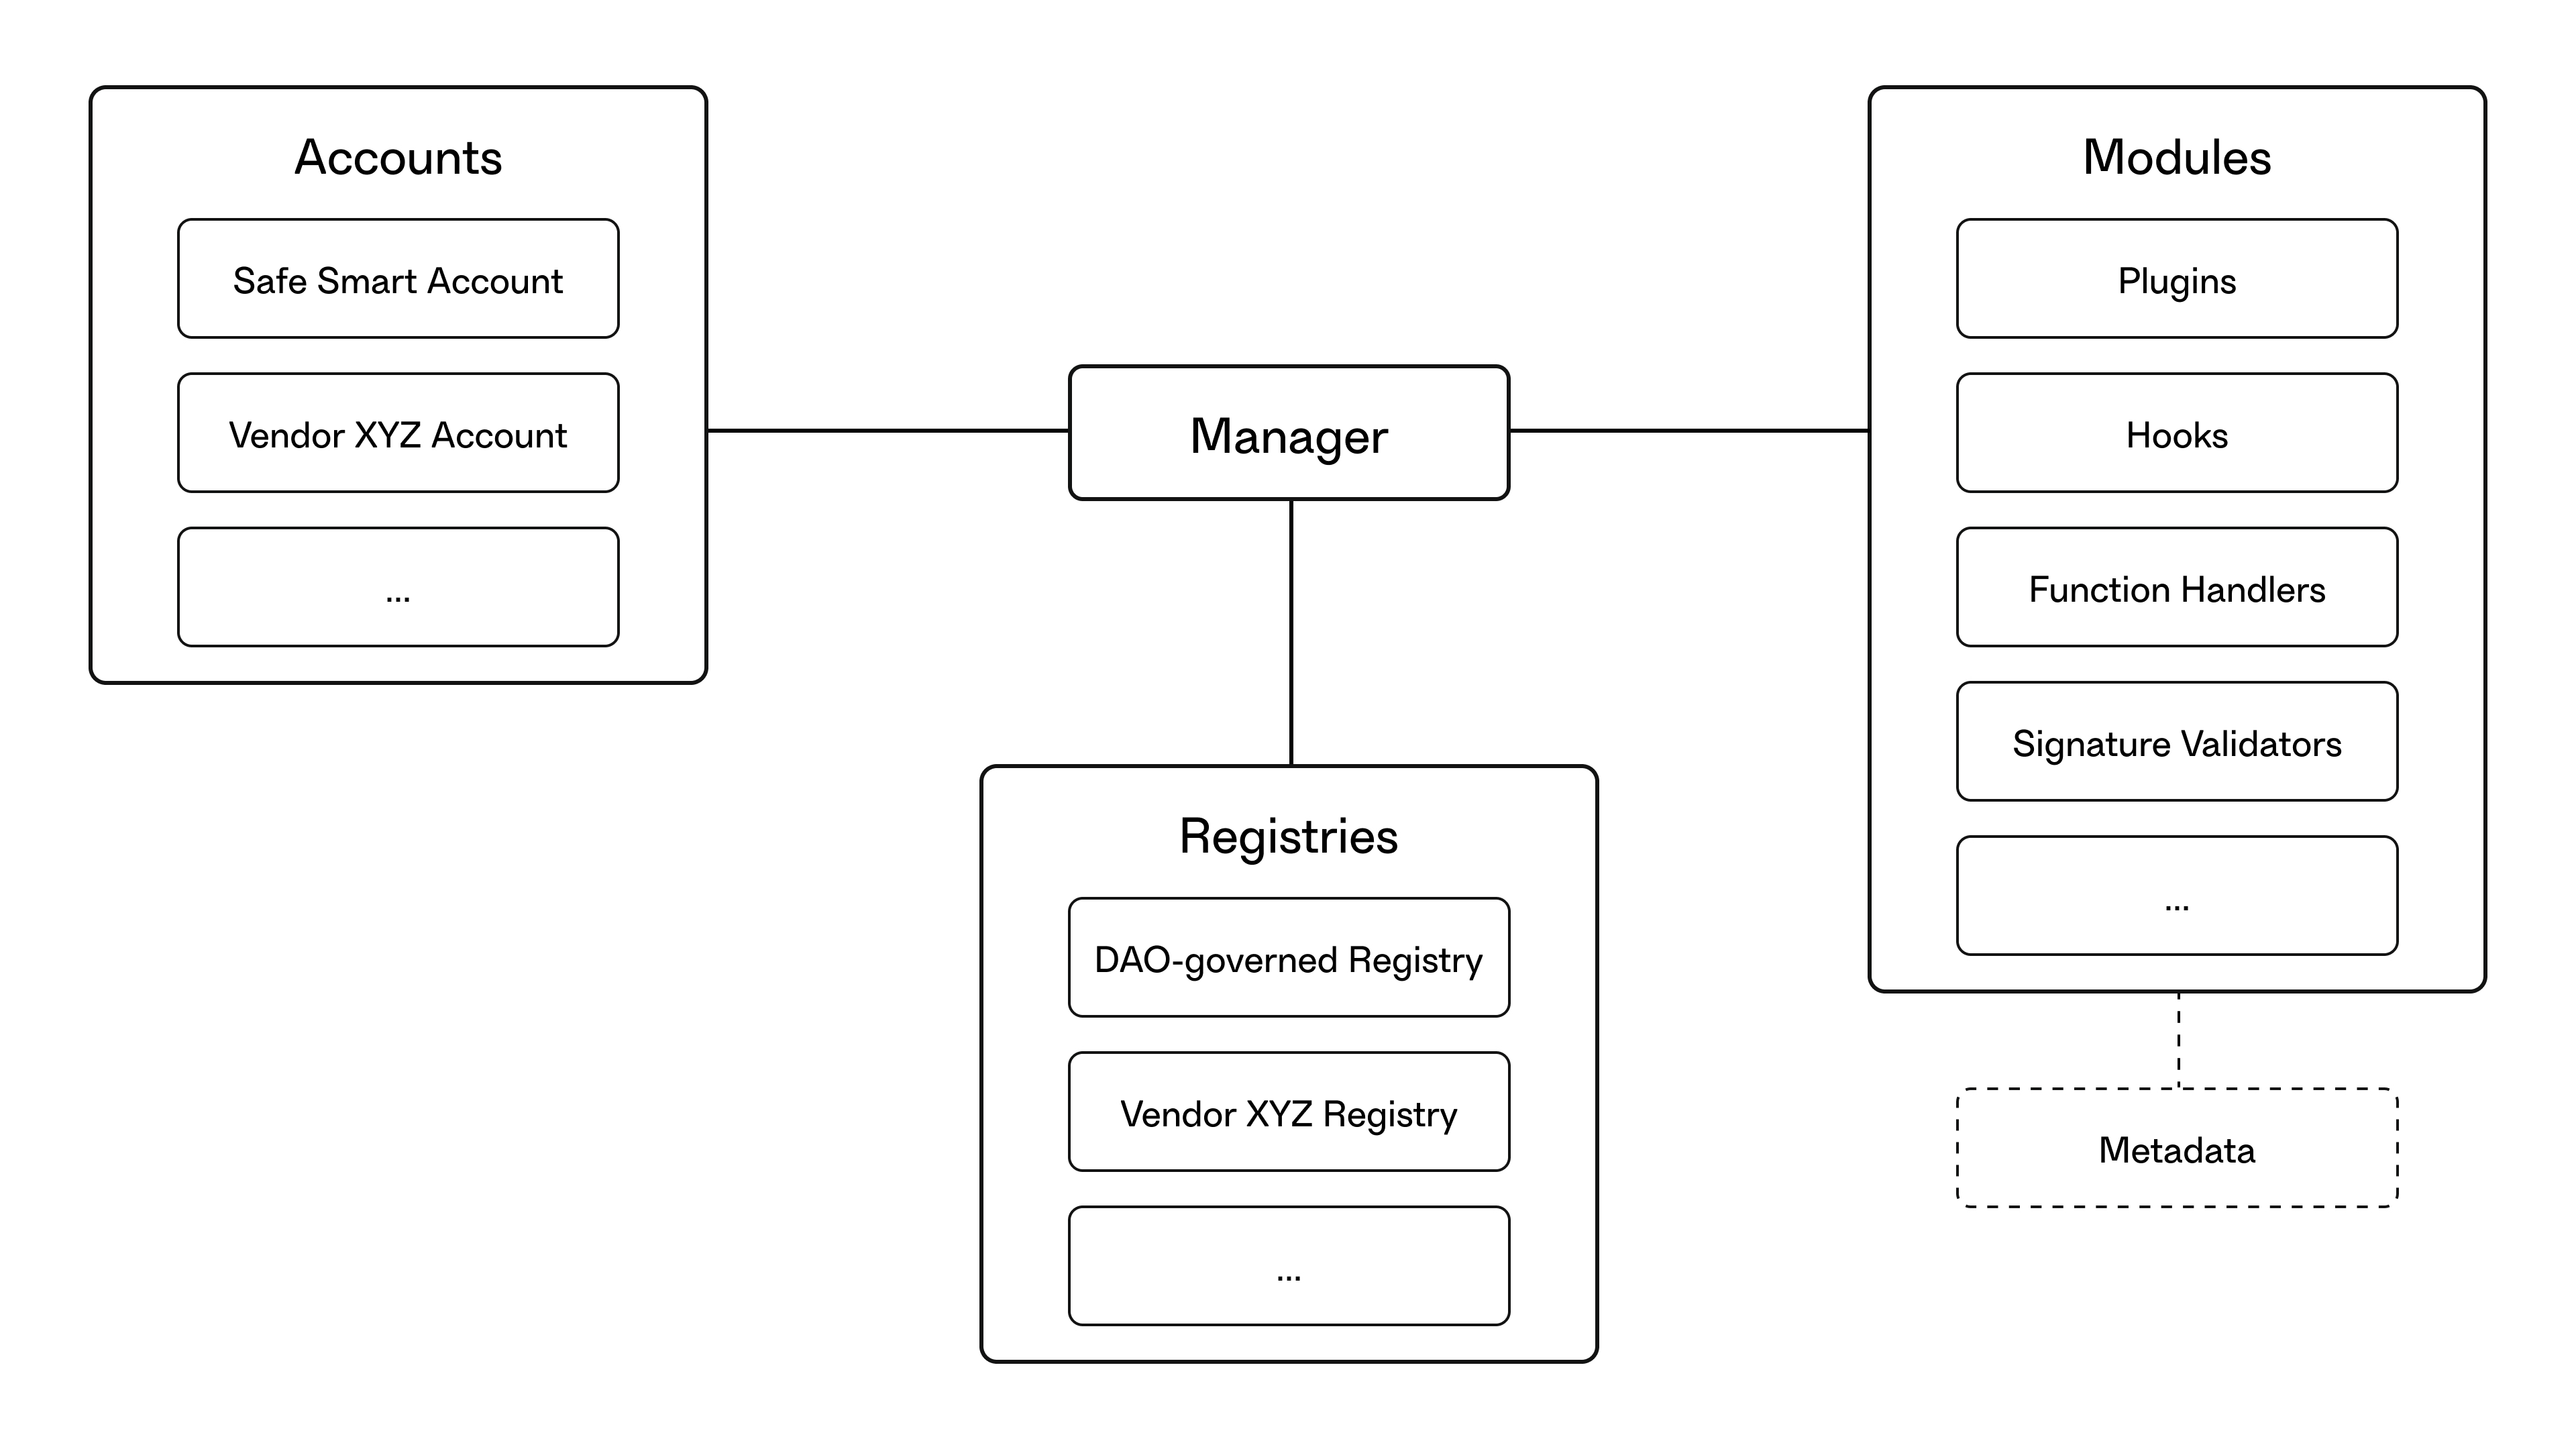
\includegraphics{graph_architecture.jpg}
  \caption{\emph{Safe\{Core\} Protocol} architecture}
  \label{fig:architecture}
\end{figure}

\hypertarget{manager}{%
  \subsection{Manager}\label{manager}}

At the center of the protocol is the \emph{Manager}, which serves as a coordination point between \emph{Accounts, Registries} and \emph{Modules} (see \emph{Figure \ref{fig:architecture}}). The \emph{Manager} implements an abstraction layer to handle the modularity of smart accounts. Users can expand the functionality of their \emph{Accounts} by activating a \emph{Registry} and enabling \emph{Modules} that are registered in the chosen \emph{Registry} (see \emph{Figure \ref{fig:activate_module}}).


\begin{figure}[h]
  \centering
  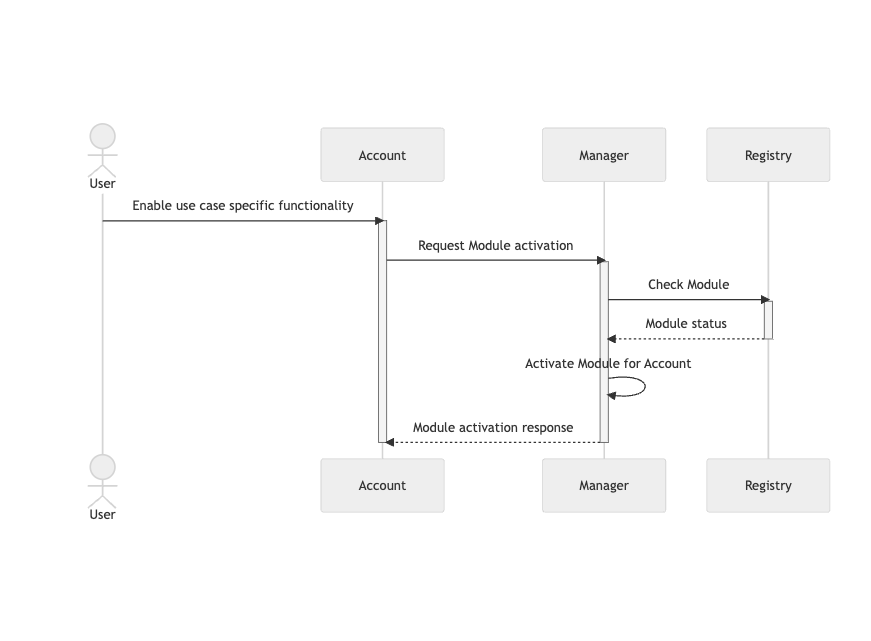
\includegraphics{graph_activate_module.png}
  \caption{\emph{Module activation flow}}
  \label{fig:activate_module}
\end{figure}

The \emph{Manager} also extends the security of smart accounts by acting as a permissioning layer, providing the ability to grant varying levels of permissions to different \emph{Modules}, such as restricting \emph{Modules} to perform configuration changes or \emph{delegatecall} operations on an \emph{Account}. Additionally, the \emph{Manager} allows implementing different default transaction fee handling schemes, such as ERC-4337, as they may vary depending on the network.

The \emph{Manager} is shared between different \emph{Accounts} and activated by the user. It is non-upgradable for security reasons, but different deployments are expected over time, adding new functionality and allowing users to migrate themselves.

\hypertarget{accounts}{%
  \subsection{Accounts}\label{accounts}}

\emph{Accounts} are user-owned smart accounts that opt-in to the protocol by enabling the \emph{Manager}, which can happen already during account deployment or when adding the first \emph{Module}. The \emph{Safe\{Core\} Protocol} is vendor-agnostic, meaning that it is not tied to a specific account implementation, as long as it supports the account interface defined by the \emph{Manager}. The initial account interface is optimized for \href{https://github.com/safe-global/safe-contracts/releases}{\uline{1.x versions of Safe Smart Account}} to expedite the development process and gather feedback. These learnings will be the foundation upon which the account interface is generalized. This will allow for a wider range of existing and new account implementations to be compatible with the protocol, and provide an open infrastructure piece for the ecosystem.

\hypertarget{modules}{%
  \subsection{Modules}\label{modules}}

\emph{Modules} extend the functionality of \emph{Accounts} in different ways. Initial module types are \emph{Plugins}, \emph{Hooks}, \emph{Signature Validators} and \emph{Function Handlers}, but additional types can be added to the \emph{Safe\{Core\} Protocol} over time. These module types are also assumed to be impacted by standards such as \href{https://eips.ethereum.org/EIPS/eip-6900}{\uline{ERC-6900}}.

\hypertarget{plugins}{%
  \subsubsection{Plugins}\label{plugins}}

\emph{Plugins} allow adding any arbitrary logic to an \emph{Account} such as recovery mechanisms, session keys and automations. These \emph{Plugins} exist as externally deployed smart contracts that are activated in the \emph{Manager} and act as alternative entry points to trigger account transactions (see \emph{Figure \ref{fig:interact_plugin}}). They can provide additional functionality for wallets, but can also be app-specific plugins that enable developers to build more powerful applications.

\hypertarget{hooks}{%
  \subsubsection{Hooks}\label{hooks}}

\emph{Hooks} add additional logic at specific points of the transaction lifecycle. The \emph{Safe\{Core\} Protocol} recognizes two types of hooks:

\begin{itemize}
  \item
        \begin{quote}
          \emph{Pre-Execution Hooks} run before a transaction is being executed.
        \end{quote}
  \item
        \begin{quote}
          \emph{Post-Execution Hooks} run at the end of a transaction.
        \end{quote}
\end{itemize}

\emph{Hooks} enable various forms of security protections, such as allow- and deny-lists, MEV and slippage protections, risk and compliance assessments, and more.

\begin{figure}[h]
  \centering
  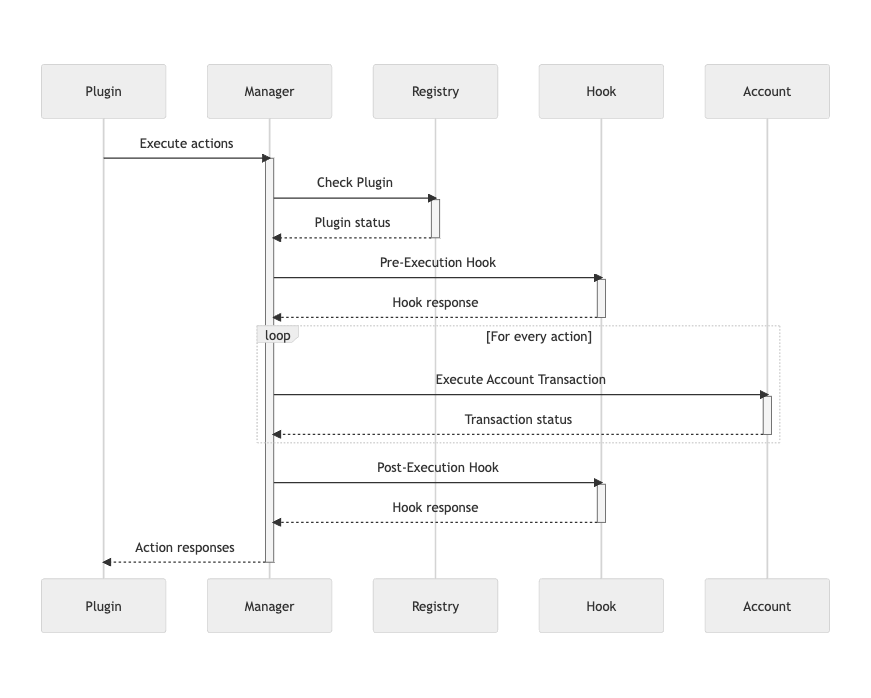
\includegraphics{graph_interact_plugin.png}
  \caption{\emph{Plugin execution flow using Hooks}}
  \label{fig:interact_plugin}
\end{figure}

\hypertarget{signature-validators}{%
  \subsubsection{Signature Validators}\label{signature-validators}}

\emph{Signature Validators} leverage the \href{https://eips.ethereum.org/EIPS/eip-1271}{\uline{ERC-1271}} standard, enabling customizable logic for (domain-based) signature validation. \emph{Signature Validators} incorporate off-chain functions, increasing the versatility of smart accounts. This also empowers intent-based architectures such as \href{https://github.com/rndlabs/cowswap-twap-orders}{\uline{CowSwap's Time-Weighted Average Price (TWAP) feature}}.

\hypertarget{function-handlers}{%
  \subsubsection{Function Handlers}\label{function-handlers}}

\emph{Function Handlers} manage arbitrary function calls when an unsupported function is called in the \emph{Account}. This enables \emph{Accounts} to contain minimal logic and remain compatible with emerging standards, such as new token types. Like all other module types, Function Handlers have to be activated with care, as even read-only functions can impact the state of the \emph{Account} if external contracts rely on them for authentication.

\hypertarget{registries}{%
  \subsection{Registries}\label{registries}}

\emph{Registries} play a critical role in establishing security guarantees and enforcing standards (e.g. \href{https://eips.ethereum.org/EIPS/eip-6900}{\uline{ERC-6900}}) for \emph{Modules}. Their role is akin to a centralized repository or an app store for smart account modules, housing a comprehensive list of approved and available \emph{Modules}. \emph{Accounts} set the registry in the \emph{Manager} and, as a result, can only activate \emph{Modules} that are approved on this specific registry.

To enhance security, \emph{Registries} can set unique inclusion/exclusion criteria and processes. For example, a \emph{Registry} may establish automated processes to detect vulnerabilities and automatically deactivates the faulty \emph{Modules} on \emph{Accounts}, potentially giving users a grace-period to overrule this decision. This allows users to benefit from the increased functionality of \emph{Modules} while maintaining high security standards.

\emph{Registries} may also enable discoverability by facilitating curation methods, serving as a convenient reference point for developers and users. For example, a \emph{Registry} may expose only those \emph{Modules} that are supported in the user interface of a specific wallet vendor to ensure stronger security and usability guarantees.

\hypertarget{metadata}{%
  \subsection{Metadata}\label{metadata}}

In order to build powerful tooling, wallets and applications on top of the \emph{Safe\{Core\} Protocol}, developers can give additional context to \emph{Modules} and module transactions as \emph{Metadata}. This allows developers to add additional information such as ``name'', ``version'', ``description'', etc. For example, developers can include a link to a frontend widget that can be leveraged as a user interface to the \emph{Module}. \emph{Registries} may use information about the version of the \emph{Module} in order to suggest updates to the user. The \emph{Metadata} can also be used to give additional context to a transaction such as which wallet vendor facilitated it.

\emph{Metadata} utilizes \href{https://eips.ethereum.org/EIPS/eip-712}{\uline{ERC-712}} to make the information machine-readable, on-chain-verifiable and semi human-readable.

\hypertarget{outlook}{%
  \section{OUTLOOK}\label{outlook}}

The above constitutes an early concept of the \emph{Safe\{Core\} Protocol} with an early reference implementation \href{https://github.com/safe-global/safe-core-protocol-specs}{\uline{being worked on}}. There are multiple pathways to develop the protocol further.

\hypertarget{fees-mechanisms}{%
  \subsection{Fees Mechanisms}\label{fees-mechanisms}}

\emph{Accounts, Registries} and \emph{Modules} should be able to charge fees, such as one-time activation fees, usage-based fees or subscription fees. These fees can be taken by the developer or shared with other stakeholders, such as wallets or \emph{Registry} maintainers. This would foster a more sustainable and vibrant smart account ecosystem by providing financial incentives to participate and contribute in the \emph{Safe\{Core\} Protocol}.

\hypertarget{chain-abstraction}{%
  \subsection{Chain Abstraction}\label{chain-abstraction}}

In the current architecture, the \emph{Safe\{Core\} Protocol} and its components have to be deployed on each chain individually. Future versions should introduce ways for protocol components to be more easily accessed cross-chain in a trust-minimized or trussless way.

\hypertarget{more-modules-types}{%
  \subsection{More Modules Types}\label{more-modules-types}}

Besides existing \emph{Modules} (\emph{Plugins}, \emph{Hooks}, \emph{Signature Validators, Function Handlers}), there could be additional module types that can be incorporated into the \emph{Safe\{Core\} Protocol} to expand the flexibility and capabilities of smart accounts. Also existing module types could be extended, such as expanding Hooks to also support plugin-specific hooks.

\hypertarget{conclusion}{%
  \section{CONCLUSION}\label{conclusion}}

The \emph{Safe\{Core\} Protocol} pioneers a modular, open-source interoperability protocol that advances the development of smart accounts, introducing a comprehensive suite of module types for enhanced functionality. Its vendor-agnostic design ensures high component reuse and maintains account portability. \emph{Registries} provide discoverability of \emph{Modules}, upholds security and interoperability standards, and facilitates vulnerability responses. Looking ahead, the protocol will evolve to accommodate chain abstraction, establish fee structures, and integrate additional module types. This work demonstrates the potential of the \emph{Safe\{Core\} Protocol} to support the EVM ecosystem's transition to smart accounts, improving developer and user experiences.

\hypertarget{section}{%
  \section{\texorpdfstring{\hfill\break}{ }}\label{section}}

\hypertarget{request-for-feedback}{%
  \section{REQUEST FOR FEEDBACK}\label{request-for-feedback}}

We invite the wider community to provide feedback to refine the \emph{Safe\{Core\} Protocol}, develop a roadmap for future iterations and build the implementation in public. A work-in-progress of the protocol specs and reference implementation can be found \href{https://github.com/safe-global/safe-core-protocol-specs}{\uline{here}}, and feedback is appreciated on \href{https://github.com/safe-global/safe-core-protocol-specs/discussions}{\uline{GitHub}} or in this \href{https://forum.safe.global/}{\uline{Forum}}. This document will be updated to incorporate feedback.

\hypertarget{acknowledgements}{%
  \section{ACKNOWLEDGEMENTS}\label{acknowledgements}}

For providing feedback on an early draft to Aaron Cook (\emph{Safe}), Anirudh Chohan (\emph{Safe}), Akshay Patel (\emph{Safe}), Andre Geest (\emph{Safe}), Auryn Macmillan (\emph{Gnosis Guild}), Bapi Reddy (\emph{Brahma}), Bil Loul (\emph{Nest Wallet}), Christoph Simmchen (\emph{Safe}), Christopher Heymann (\emph{1kx}), Clement Bihorel (\emph{Safe}), Daniel Fischmann (\emph{L1D}), Daniel Partida (\emph{Safe}), Eylon Aviv (\emph{Collider}), Frederico Sabino (\emph{Safe}), Ivo Georgiev (\emph{Ambire Wallet}), Jan Baeriswyl (\emph{very early Ventures}), John Ennis (\emph{Safe}), Jonah Ehrlich (\emph{Den}), Josef Gattermayer (\emph{Ackee Blockchain}), Kurt Larsen (\emph{Rhinestone}), Lefteris Karapetsas (\emph{Rotki}), Marvin Lin (\emph{Gnosis Guild}), Micah Zoltu (\emph{serv.eth}), Nichanan Kesonpat (\emph{1kx}), Poolpi Tako (\emph{Yearn}), Robert Koschig (\emph{1kx}), Sebastian Bürgel (\emph{Hopr}), Stefan George (\emph{Gnosis}), Steven Biekens (\emph{Safe}), Tobias Schubotz (\emph{Safe}), Vitaly Bahachuk (\emph{Linen Wallet}).

\end{document}
